\section{Questions à choix multiple \textit{(5 points)}}

Cet exercice se présente sous la forme d'un questionnaire à choix multiple (QCM). Les cinq questions sont indépendantes. Pour chaque question, une seule réponse est exacte, on demande d'indiquer cette réponse sans la justifier. Chaque bonne réponse rapporte 1 point, chaque réponse incorrecte retire \num{0.25} point, une question sans réponse n'apporte ni ne retire aucun point.

\begin{questions}
	\question[1] On considère la suite arithmétique $(u_n)$, telle que $u_0 = 16$ et $u_4 = -4$. La raison de la suite $(u_n)$ est :
	
	\begin{oneparcheckboxes}
		\choice \num{3.5};
		\choice \num{3};
		\choice \num{-3};
		\CorrectChoice \num{-5}.
	\end{oneparcheckboxes} 

	\question[1] On considère la suite $(u_n)$ telle que $u_n = 3n - 2$. La suite $(u_n)$ est :
	
	\begin{checkboxes}
		\choice une suite arithmétique de raison \num{-2};
		\choice une suite géométrique de raison \num{3};
		\correctchoice une suite arithmétique de raison \num{3};
		\choice une suite géométrique de raison \num{2}.
	\end{checkboxes}

	\question[1] On injecte $u_0$ cm$^3$ d'un médicament dans le sang d'un patient. La quantité de ce médicament présente dans le sang du patient $n$ heures après l'injection est $u_n$. La quantité de médicament présente dans le sang baisse de 20 \% chaque heure.
	La suite $(u_n)$ est :
	
	\begin{checkboxes}
		\choice une suite arithmétique de raison \num{-20};
		\choice une suite géométrique de raison \num{1.20};
		\choice une suite arithmétique de raison \num{-0.2};
		\correctchoice une suite géométrique de raison \num{0.8}.
	\end{checkboxes}

	\question[1] On reprend la situation décrite dans la question 3. Cinq heures après l'injection, il reste dans le sang du patient environ :
	
	\begin{checkboxes}
		\choice \num{67} \% de la quantité injectée ;
		\choice \num{20} \% de la quantité injectée ;
		\choice rien ;
		\CorrectChoice \num{33} \% de la quantité injectée.
	\end{checkboxes}

 
	
		
	
	\question[1] 
	\begin{multicols}{2}
		
		La feuille de calcul ci-dessous est utilisée pour calculer les premiers termes de la suite géométrique $(u_n)$ de premier terme \num{5000} et de raison \num{1.02}. La formule à entrer dans la cellule B3 et à recopier vers le bas est :
	
	\begin{oneparcheckboxes}
		\choice $\num{5000}*\num{1.02}$;
		\choice $=\$B\$2^*\num{1.02}$; \ \  \ 
 		\correctchoice $=B2^*\num{1.02}$;
		\choice $=\num{1.02} \hat{\ } A3$;
	\end{oneparcheckboxes}

	\begin{center}
		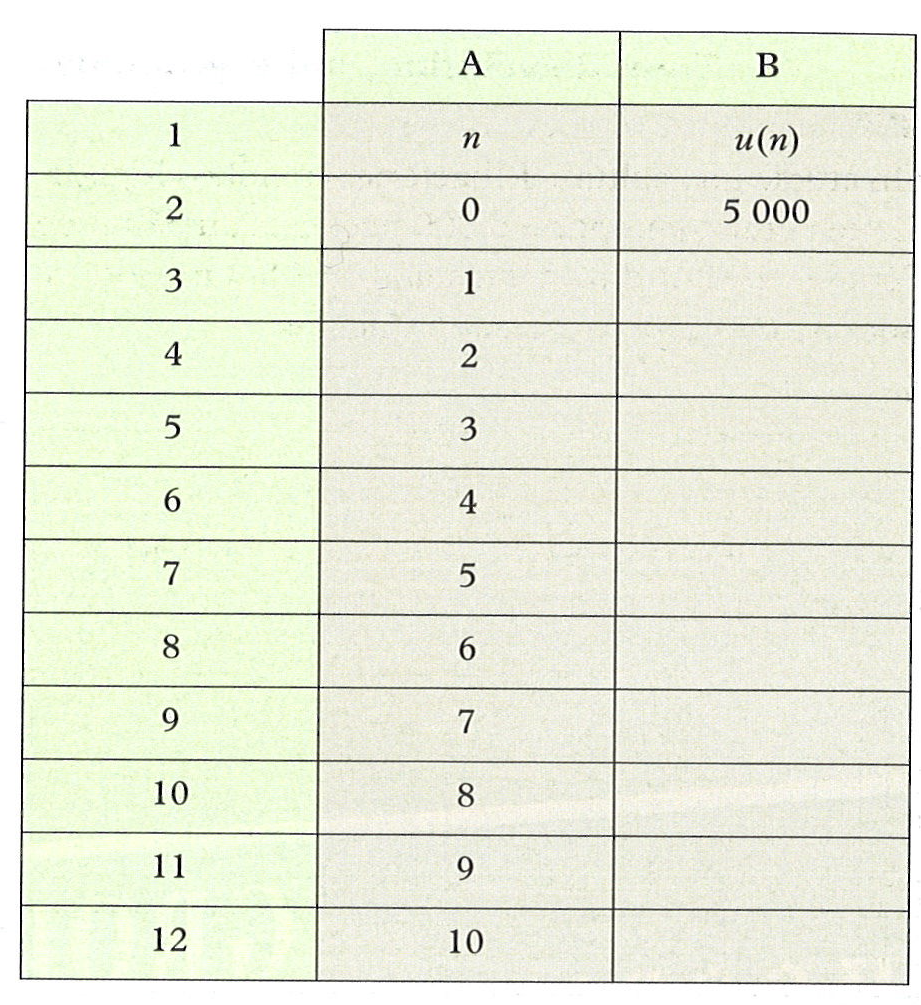
\includegraphics[scale=0.8]{qcm}
	\end{center}
	
	\end{multicols}
\end{questions}  